\documentclass{article}

\usepackage{graphicx}
\usepackage{tikz}
\usepackage{tikzsymbols}
\usetikzlibrary{calc,patterns,shapes.geometric}
\pagestyle{empty}
\usepackage[margin=0pt]{geometry}
\geometry{papersize={14in,12in}}

\def\centerarc[#1](#2)(#3:#4:#5){\draw[#1] ($(#2)+({#5*cos(#3)},{#5*sin(#3)})$) arc (#3:#4:#5);}

\begin{document}
	\begin{figure}
		\centering
		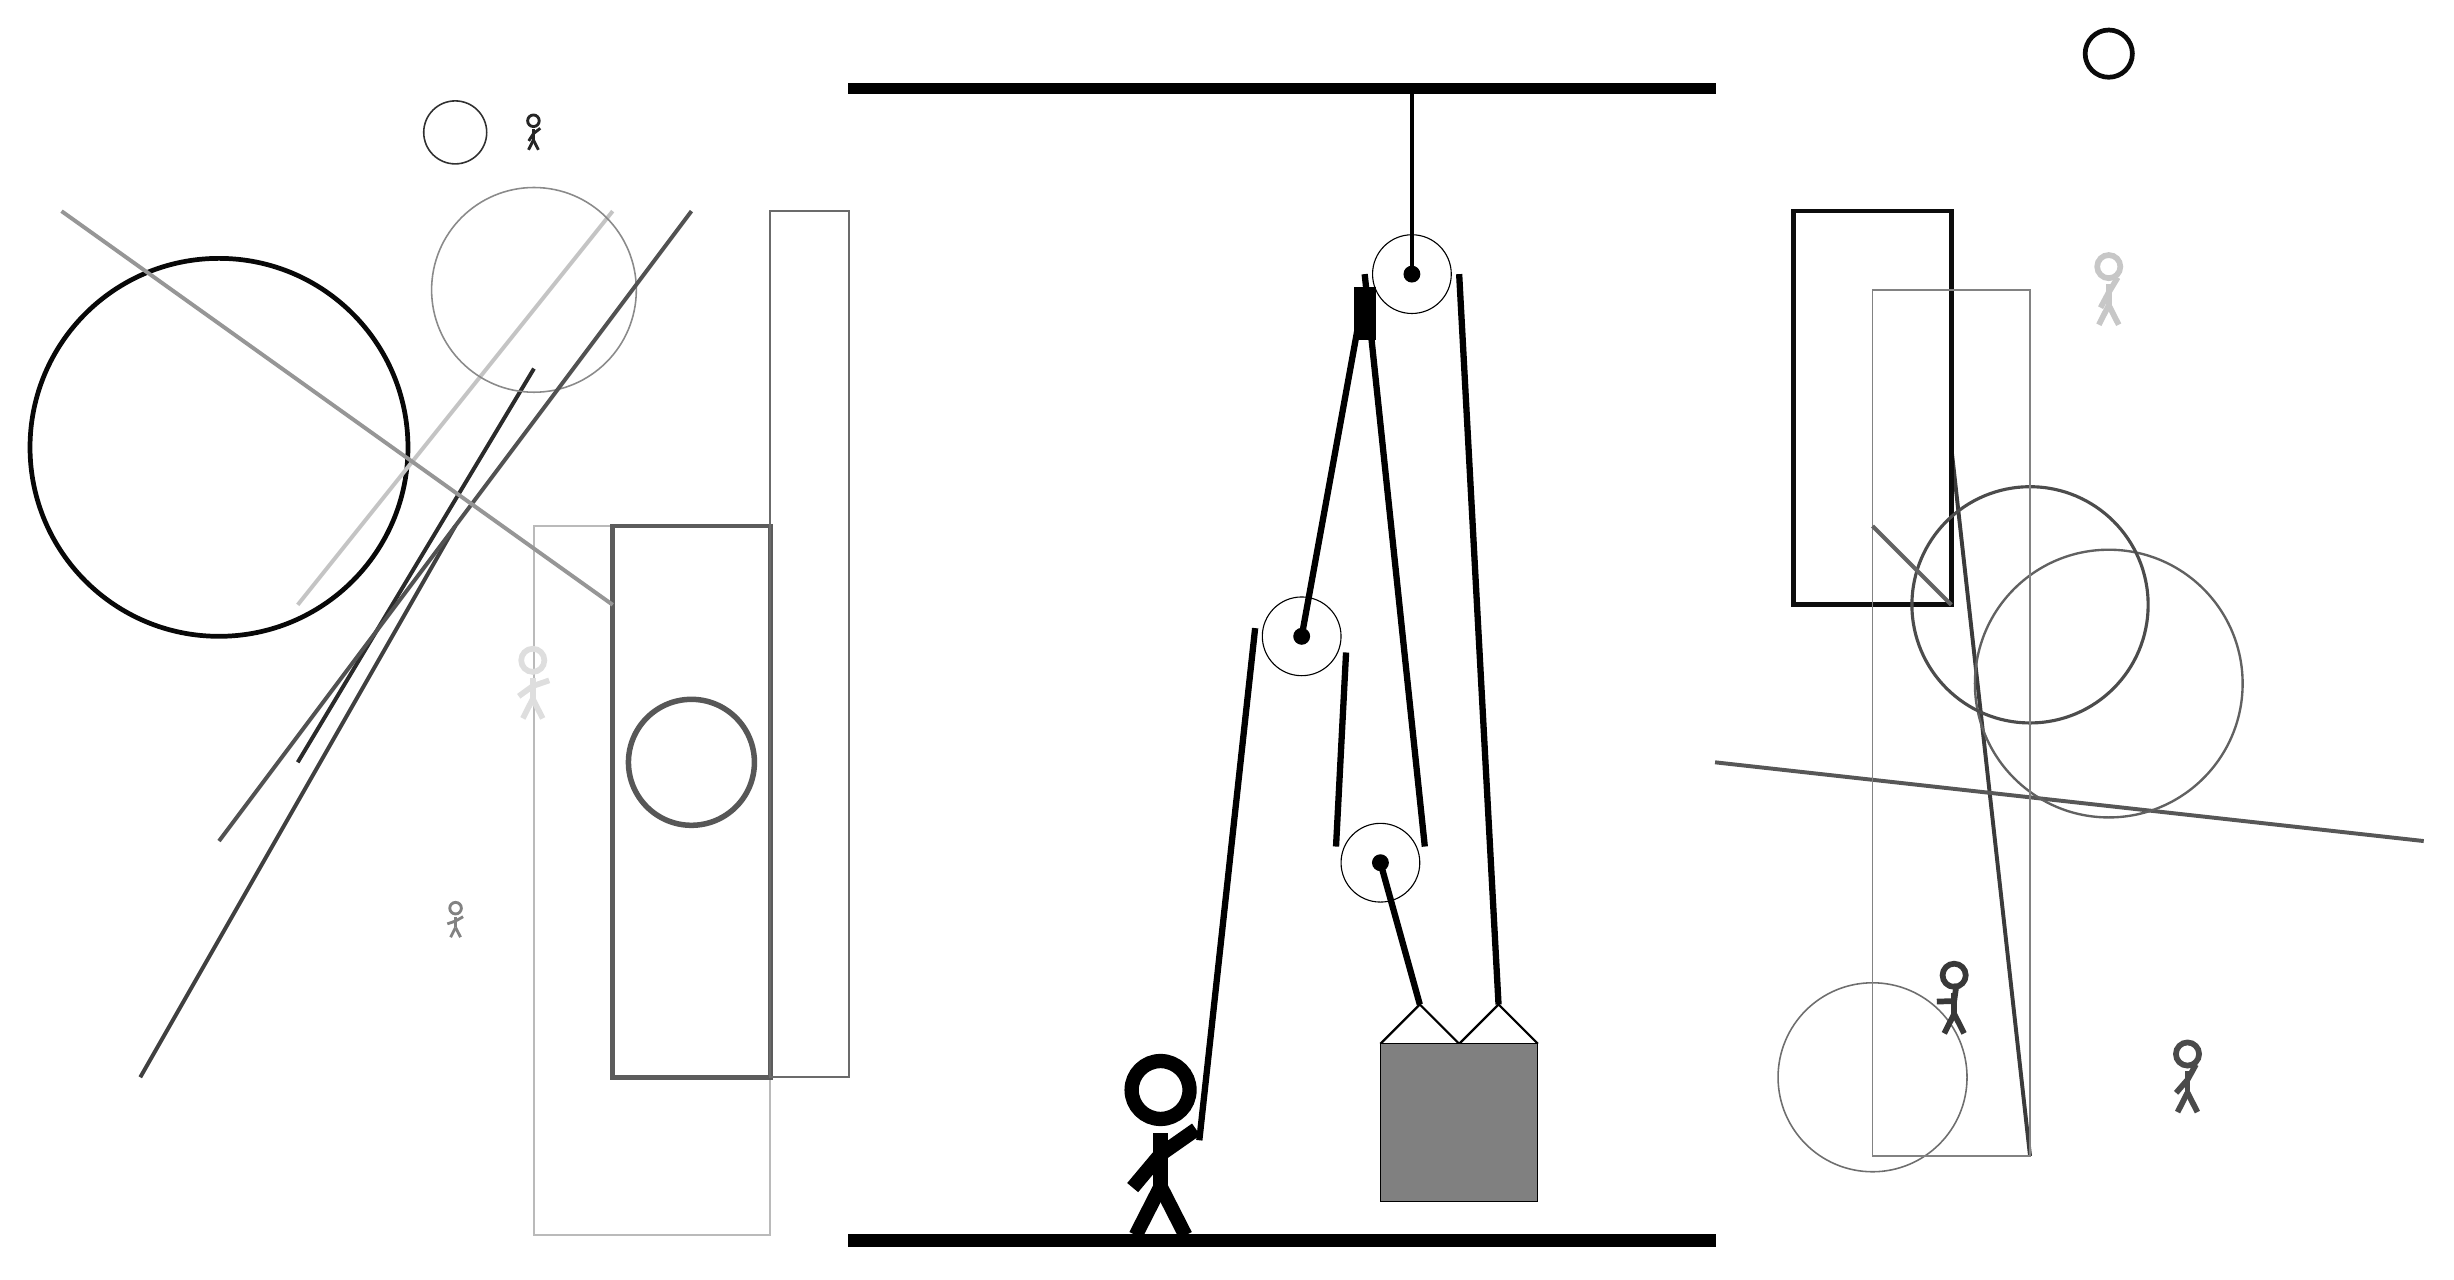
\begin{tikzpicture}
			%%%%% START %%%%%
			
			\draw[fill=black] (-6, 11.5) rectangle (5, 11.625);
			
			\draw (-0.25, 4.6) circle (0.5);
			\draw[fill=black] (-0.25, 4.6) circle (0.1);
			
			\draw (0.75, 1.725) circle (0.5);
			\draw[fill=black] (0.75, 1.725) circle (0.1);
			
			\draw (1.15, 9.2) circle (0.5);
			\draw[fill=black] (1.15, 9.2) circle (0.1);
			\draw[very thick] (1.15, 9.2) -- (1.15, 11.5);
			
			\draw[line width=0.5mm, color=black!77](8, 7) -- (9, -2);
			
			\draw [line width=0.7mm, color=black!66](-8, 3) circle (0.8);
			\draw [line width=0.2mm, color=black!81](-11, 11) circle (0.4);
			\draw[line width=0.3mm, color=black!27] (-7, 6) rectangle (-10, -3);
			\draw [line width=0.2mm, color=black!57](7, -1) circle (1.2);
			\draw[line width=0.5mm, color=black!66](5, 3) -- (14, 2);
			
			\node[line width=0.7mm, color=black!49] at (-11, 1) {\Strichmaxerl[2][19][30]};
			\draw[line width=0.6mm, color=black!95] (6, 5) rectangle (8, 10);
			\draw [line width=0.3mm, color=black!62](10, 4) circle (1.7);
			\draw[line width=0.5mm, color=black!83](-10, 8) -- (-13, 3);
			\draw [line width=0.6mm, color=black!97](-14, 7) circle (2.4);
			
			\draw [line width=0.4mm, color=black!70](9, 5) circle (1.5);
			\node[line width=0.3mm, color=black!78] at (8, 0) {\Strichmaxerl[4][2][82]};
			
			\draw[line width=0.5mm, color=black!23](-9, 10) -- (-13, 5);
			\node[line width=0.7mm, color=black!13] at (-10, 4) {\Strichmaxerl[4][36][19]};
			\node[line width=0.5mm, color=black!71] at (11, -1) {\Strichmaxerl[4][49][61]};
			\node[line width=0.7mm, color=black!22] at (10, 9) {\Strichmaxerl[4][62][59]};
			\draw[line width=0.2mm, color=black!49] (7, -2) rectangle (9, 9);
			\draw[line width=0.5mm, color=black!75](-11, 6) -- (-15, -1);
			\draw [line width=0.2mm, color=black!46](-10, 9) circle (1.3);
			\draw[line width=0.5mm, color=black!68](-8, 10) -- (-14, 2);
			
			\draw[line width=0.6mm, color=black!64] (-7, -1) rectangle (-9, 6);
			\node[line width=0.4mm, color=black!85] at (-10, 11) {\Strichmaxerl[2][57][38]};
			\draw[line width=0.5mm, color=black!41](-9, 5) -- (-16, 10);
			\draw[line width=0.5mm, color=black!61](8, 5) -- (7, 6);
			\draw [line width=0.6mm, color=black!96](10, 12) circle (0.3);
			
			\draw[line width=0.2mm, color=black!58] (-6, -1) rectangle (-7, 10);
			
			\draw[thick]  (0.75, -0.575) -- (1.25, -0.075) -- (1.75, -0.575) -- (2.25, -0.075) -- (2.75, -0.575);
			\draw[fill=black!50] (0.75, -0.575) rectangle (2.75, -2.575);
			
			\draw[line width=0.8mm] (-0.25, 4.6) -- (0.55, 9.0);
			\draw[line width=0.8mm, fill=black](0.45, 8.4) rectangle (0.65, 9.0);
			\draw[line width=0.8mm] (-1.55, -1.8) -- (-0.8409, 4.7042);
			\centerarc[line width=0.8mm](-0.25, 4.6)(-20:170:0.6);
			\draw[line width=0.8mm] (0.3138, 4.3948) -- (0.1862, 1.9302);
			\centerarc[line width=0.8mm](0.75, 1.725)(160:380:0.6);
			\draw[line width=0.8mm] (1.3138, 1.9302) -- (0.55, 9.2);
			\draw[line width=0.8mm](0.75, 1.725) -- (1.25, -0.075);
			\centerarc[line width=0.8mm](1.15, 9.2)(0:180:0.6);
			\draw[line width=0.8mm] (1.75, 9.2) -- (2.25, -0.075);
			
			\node at (-2, -1.9) {\Strichmaxerl[10][50][35]};
			
			\draw[fill=black] (-6, -3) rectangle (5, -3.15);
			
			%%%%% END %%%%%
		\end{tikzpicture}
	\end{figure}	
\end{document}